\documentclass[12pt,a4paper,oneside]{report}

% --- Encodage et Langue ---
\usepackage[T1]{fontenc}
\usepackage[utf8]{inputenc}
\usepackage{csquotes}
\usepackage[english,french]{babel}
\usepackage{lmodern}
\usepackage{microtype}

% --- Mise en page (Geometry) ---
\usepackage{geometry}
\geometry{
  a4paper,
  top=25mm,
  bottom=25mm,
  left=30mm,      % Marge gauche exigée à 30 mm
  right=30mm,     % Marge droite exigée à 30 mm
  footskip=15mm   % Positionne le numéro de page à 10 mm du bord inférieur (25mm - 15mm)
}

% --- Interlignes et Indentation française ---
\usepackage{setspace}
\onehalfspacing                  % Corps du texte en interligne 1,5
\setlength{\parindent}{1cm}     % Alinéa de 1 cm (norme classique)
\setlength{\parskip}{0pt}       % Pas d'espace blanc entre les paragraphes

% --- Notes de bas de page ---
\usepackage[hang,flushmargin]{footmisc}
\renewcommand{\footnotesize}{\fontsize{9}{11}\selectfont} % Notes à 9pt (min 8pt)

% --- Mathématiques ---
\usepackage{amsmath, amssymb, amsfonts}
\usepackage{siunitx}
\sisetup{output-decimal-marker = {,}} % Configure siunitx pour utiliser la virgule française

% --- Graphiques et Tableaux ---
\usepackage{graphicx}
\usepackage{caption}
\usepackage{subcaption}
\usepackage{booktabs} % Pour de beaux tableaux
\usepackage{multirow} % Pour fusionner des lignes si nécessaire
\usepackage{array}

% --- En-têtes et Pieds de page ---
\usepackage{fancyhdr}
\pagestyle{fancy}
\fancyhf{}
\fancyfoot[C]{\thepage} % Numéro de page centré en bas
\renewcommand{\headrulewidth}{0pt}
\renewcommand{\footrulewidth}{0pt}

\fancypagestyle{plain}{
  \fancyhf{}
  \fancyfoot[C]{\thepage}
  \renewcommand{\headrulewidth}{0pt}
  \renewcommand{\footrulewidth}{0pt}
}

% --- Titres des sections ---
\usepackage{titlesec}

% 1. Pour les chapitres numérotés (avec ligne fine et grand "Chapitre X")
\titleformat{\chapter}[display]
{\normalfont}
{\LARGE\bfseries\chaptername\ \thechapter}
{2em}
{\titlerule[0.4pt]\vspace{2em}\centering\LARGE\bfseries}

% 2. Pour les chapitres non numérotés (Introduction, Conclusion, etc. sans ligne fine)
\titleformat{name=\chapter,numberless}[display]
{\normalfont}
{}
{0pt}
{\centering\huge\bfseries}

% Espacement vertical global des chapitres
\titlespacing*{\chapter}{0pt}{0pt}{40pt}

% --- Hyperliens ---
\usepackage[colorlinks=true, allcolors=black]{hyperref}

% --- Bibliographie (BibLaTeX) ---
\usepackage[
  backend=biber,
  style=apa,
  language=french
]{biblatex}

% Associe les règles de langue française spécifiques à l'APA
\DeclareLanguageMapping{french}{french-apa}

% Optionnel : met le "et al." en italique
\DefineBibliographyStrings{french}{andothers = {\textit{et~al.}}}
\addbibresource{bibliography/references.bib}

% --- Environnement pour les citations longues (Long quote) ---
\newenvironment{longquote}{
  \begin{list}{}{
      \setlength{\leftmargin}{10mm}  % Retrait de 10 mm à gauche
      \setlength{\rightmargin}{10mm} % Retrait de 10 mm à droite
      \setlength{\topsep}{0.5em}     % Petit espace vertical avant/après
    }
    \item[]
          \singlespacing                   % Interligne 1,0 forcé
          }{
  \end{list}
}

\title{Indexation sémantique frugale des actes d'état civil manuscrits~: graphe de connaissances au service de l'archivage et de la gouvernance documentaire en Afrique subsaharienne}
\author{Ousmane Hamadou}
\date{\today}

\begin{document}

% --- Front Matter (Chiffres romains) ---


% 1. Page de titre
\begin{titlepage}
    \thispagestyle{empty}
    \begin{center}
        {\Large\bfseries Université de Ngaoundéré}\\[0.4cm]
        {\large \textsc{Facult\'e des Sciences}}\\[0.2cm]
        {\normalsize Département d'Informatique}\\[2.5cm]

        {\Large\bfseries Indexation sémantique frugale des actes d'état civil manuscrits~:  graphe de connaissances au service de l'archivage et de la gouvernance documentaire en Afrique subsaharienne}\\[2cm]

        Mémoire présenté en vue de l'obtention du diplôme de\\[0.3cm]
        {\bfseries Master 2 en Informatique}\\[0.3cm]
        Spécificité : SLED\\[2cm]

        Par :\\[0.3cm]
        {\large\bfseries Ousmane Hamadou}\\[0.5cm]  % Correction ici : \\ au lieu de \[
        Titulaire d'une Licence en Mathématiques et Informatique\\[2cm]

        Sous la direction de :\\[0.3cm]
        {\bfseries Pr Fendji Jean Louis}\\[2.5cm]

        {\itshape Année académique 2025/2026}
    \end{center}
\end{titlepage}

\pagenumbering{roman}
\setcounter{page}{2}
\clearpage
\chapter*{Résumé}
\addcontentsline{toc}{chapter}{Résumé}
\thispagestyle{plain} % Force l'affichage du numéro de page en bas

\begin{otherlanguage*}{french}
    % Votre texte de résumé en français ici...

    \vspace{1em}
    \noindent\textbf{Mots-clés :} Indexation sémantique, Graphe de connaissances, Frugalité, Actes d'état civil.
\end{otherlanguage*}
\clearpage
\chapter*{Abstract}
\addcontentsline{toc}{chapter}{Abstract}
\thispagestyle{plain} % Force l'affichage du numéro de page en bas

\begin{otherlanguage*}{english}
    % Your English abstract text here...

    \vspace{1em}
    \noindent\textbf{Keywords:} Semantic indexing, Knowledge graph, Frugality, Civil status records.
\end{otherlanguage*}

\selectlanguage{french}
\clearpage
\phantomsection % Assure une ancre correcte pour le lien hypertexte
\addcontentsline{toc}{chapter}{\contentsname}
\tableofcontents
\listoffigures
\listoftables

\chapter*{Dédicace}
\addcontentsline{toc}{chapter}{Dédicace}

\begin{center}
    \textit{À ma famille, à tous ceux qui m'ont soutenu dans ce parcours de recherche...}
\end{center}
\chapter*{Remerciements}
\addcontentsline{toc}{chapter}{Remerciements}

% Remerciements à venir

% --- Main Matter (Chiffres arabes) ---
\pagenumbering{arabic}
\setcounter{page}{1}

\chapter*{Introduction}
\addcontentsline{toc}{chapter}{Introduction}

\begin{longquote}
    Les Buts de la Documentation organisée consistent à pouvoir offrir sur tout ordre de fait et de connaissance des informations documentées : 1\textdegree{} universelles quant à leur objet ; 2\textdegree{} sûres et vraies ; 3\textdegree{} complètes ; 4\textdegree{} rapides ; 5\textdegree{} à jour ; 6\textdegree{} faciles à obtenir ; 7\textdegree{} réunies d'avance et prêtes à être communiquées ; 8\textdegree{} mises à la disposition du plus grand nombre. \parencite{otletTraiteDocumentationLivre2021}
\end{longquote}

\begin{longquote}
    Les archives constituent un patrimoine unique et irremplaçable transmis de génération en génération [...].
    Sources d'informations fiables pour une gouvernance responsable et transparente, [elles] jouent un rôle essentiel dans le développement des sociétés. \parencite{UniversalDeclarationArchives}
\end{longquote}

Ces deux textes définissent le contrat social de l'archivistique moderne : transformer la trace brute en connaissance organisée, universellement accessible et durablement fiable.
Pres de un siècle après Otlet, cette ambition s'est déplacée vers le Web sémantique et les graphes de connaissances --- seuls capables aujourd'hui de tenir la promesse d'une information structurée au-delà du document isolé.
En Afrique subsaharienne pourtant, cet idéal se heurte à une réalité matérielle qui impose d'intégrer une dimension absente des paradigmes dominants des pays Nord : la frugalité.

\subsubsection{Contexte et motivation}

L'Afrique subsaharienne connaît une accélération de la transformation numérique de ses administrations publiques \parencite{lawalDIGITALGOVERNANCEINCLUSIVE2025,egbeleoDigitalTransformationInstitutional2025}.
Dans cette dynamique, l'enregistrement des faits d'état civil s'impose comme une infrastructure de gouvernance, d'inclusion sociale et de souveraineté nationale \parencite{BirthRegistrationSubSaharan2025} : garantir à chaque individu une existence légale, conformément à l'Objectif de Développement Durable 16.9 des Nations Unies, conditionne toute planification en matière d'éducation, de santé et de droits fondamentaux.
Or la gestion documentaire de la région fait face à une crise silencieuse d'amnésie de ses passifs archivistiques : la production administrative, bien qu'indispensable, a longtemps été gérée de manière inadéquate, mettant à risque la préservation de la mémoire collective et la justification des droits individuels \parencite{michaudSecretsDEtats2015, bintsenaArchivesAdministrativesDans2017}.

Plusieurs pays de la sous-région illustrent cette tension entre ambition de modernisation et réalité de terrain.
Le Sénégal est parvenu à numériser plus de 20 millions d'actes via le projet NEKKAL \parencite{civipol2023nekkal}, ce modèle reposait sur des moyens financiers et humains extrêmement lourds --- subventions internationales et indexation manuelle massive ---, rendant sa reproduction problématique pour les États aux ressources plus limitées.
Le Burkina Faso a déployé iCivil, un système d'enregistrement nativement numérique --- tourné vers le flux des actes à venir, non vers l'indexation rétrospective du stock hérité.
En 2024, le Cameroun a engagé un tournant normatif majeur par l'adoption simultanée de lois régissant les archives numériques (n° 2024/001), l'état civil (n° 2024/016) et la protection des données personnelles (n° 2024/017).
Cependant, ce nouvel élan juridique se heurte à d'importantes contraintes du terrain : un déficit documentaire touchant près de 7 millions d'individus et la sous-exploitation d'un patrimoine d'actes manuscrits anciens restreint à des \og îlots informationnels \fg{} locaux \parencite{olembe2024webinaire}.
Nous n'avons pas identifié, dans la littérature et les sources institutionnelles consultées, de dispositif documenté combinant aujourd'hui numérisation de masse et indexation sémantique du stock manuscrit hérité --- c'est précisément ce vide que ce mémoire investit.

Cette même tension se lit au niveau des standards de description archivistique. Les modèles hérités --- OAIS, EAD, Dublin Core --- structurent un fonds selon une logique arborescente à racine unique, inapte à représenter un acte d'état civil mettant simultanément en jeu plusieurs agents et référencé par d'autres actes ultérieurs.
Le standard Records in Contexts (RiC) publié par le Conseil international des archives, dépasse cette rigidité en substituant à l'arbre un graphe de relations typées --- mais cette bascule ne résout ni l'indexation du contenu de ces documents manuscrits, ni le coût des ressources qu'exige son déploiement effectif.

Les systèmes documentaires classiques reposent majoritairement sur une indexation lexicale ou contrôlée, fondée sur des mots-clés, des descripteurs, des classifications ou des thésaurus \parencite{menilletThesaurusIndexation1993}, ce qui les rend moins aptes à représenter des relations complexes se limitant à retrouver des documents contenant certains mots, non des faits : une requête portant sur une même lignée familiale n'y a simplement pas de formulation possible.
L'indexation sémantique par graphe de connaissances offre une réponse structurelle en représentant chaque personne comme un nœud persistant à travers les actes.
Cette expressivité a un double coût : un graphe ne dissout pas le bruit de la reconnaissance manuscrite, il le déplace vers un problème de résolution d'entités \parencite{alkendiAdvancementsChallengesHandwritten2024,tuselmannNamedEntityLinking2022}, et son déploiement mobilise une infrastructure de calcul dont la plupart des services d'archives subsahariens ne disposent pas, au risque d'une dépendance technologique exogène menaçant la souveraineté numérique des États sur leurs données d'identité \parencite{musoniDigitalIDSystems}.


\subsubsection{Question de recherche principale}
C'est de cette confrontation --- une solution conceptuellement adéquate mais de ressource inaccessible --- que ce mémoire pose ainsi la question suivante :

\emph{Dans quelle mesure l'intégration de techniques de traitement automatique des langues frugales permet-elle de valider la viabilité d'un modèle de graphe de connaissances normalisé (RiC-O) pour la préservation et l'exploitation des archives manuscrites d'état civil en Afrique subsaharienne, en milieu à ressources computationnelles limitées ?}

Plus spécifiquement, ce mémoire évalue si une mobilisation des modèles de langue frugaux plutôt que leurs homologues industriels, des méthodes d'adaptation elles-mêmes économes en données annotées et une exécution intégrale sur infrastructure strictement frugale est compatible avec une qualité sémantique satisfaisante.

\subsubsection{Questions de recherche secondaires}

Cette viabilité se décline en quatre Questions de recherche (QRs) :



: quelle est la corrélation entre la variabilité des écritures cursives administratives subsahariennes et la fiabilité des transcriptions automatiques au sein d'un pipeline frugal ? (Q1\label{ques:1}). La deuxième interroge la modélisation : comment adapter l'ontologie RiC-O aux structures de parenté et de filiation propres aux contextes subsahariens sans rompre l'interopérabilité internationale du standard ? (Q2\label{ques:2}). La troisième s'attaque au cœur du compromis technique : quelles sont les limites de performance des modèles de langue frugaux dans l'extraction de relations complexes depuis un texte administratif manuscrit bruité ? (Q3\label{ques:3}). Enfin, la dernière évalue une stratégie de mitigation : une architecture d'extraction hybride, combinant règles symboliques et modèle statistique frugal, améliore-t-elle la robustesse du pipeline par rapport à un modèle neuronal utilisé seul ? (Q4\label{ques:4}).

À ces questions répondent quatre hypothèses de recherche, conçues comme des postulats falsifiables. Un graphe de connaissances conforme à RiC-O réduit significativement les silences documentaires liés aux variantes onomastiques, comparativement à une indexation lexicale classique (H1\label{hypo:1}). Une quantification INT8 des modèles frugaux mobilisés n'entraîne pas de dégradation critique de leur performance d'extraction, tout en rendant possible une exécution intégrale sur infrastructure CPU (H2\label{hypo:2}). Un profil d'application RiC-O simplifié et adapté aux structures de parenté subsahariennes représente des fonds hétérogènes sans recourir à une centralisation matérielle lourde (H3\label{hypo:3}). Enfin, une stratégie hybride combinant règles symboliques et modèle statistique frugal améliore la robustesse de l'extraction sur texte administratif bruité, comparativement à un modèle neuronal frugal utilisé seul (H4\label{hypo:4}).

Conformément au paradigme de la Design Science Research \parencite{hevnerDesignScienceInformation,Peffers2007ADS}, cette recherche distingue des objectifs scientifiques, orientés vers la production de connaissances généralisables, et des objectifs opérationnels, orientés vers la conception de l'artefact qui sert de support empirique à cette évaluation. Les objectifs scientifiques sont au nombre de trois : caractériser les limites de scalabilité sémantique de RiC-O dans un environnement de calcul dégradé appliqué au patrimoine manuscrit subsaharien (OS1) ; modéliser un profil RiC-O adaptable aux particularités juridiques, onomastiques et parentales des administrations d'Afrique subsaharienne (OS2) ; et évaluer empiriquement l'impact du bruit de transcription HTR sur la robustesse des requêtes SPARQL et sur la qualité du graphe produit (OS3). Les objectifs opérationnels visent la conception de l'artefact : concevoir et implémenter, sur un corpus de preuve de concept de 50 à 100 actes manuscrits camerounais numérisés par photographie, un pipeline frugal complet articulant HTR, extraction d'entités et de relations, et peuplement d'un graphe RiC-O (OO1) ; fine-tuner et quantifier des modèles frugaux exécutables sur infrastructure strictement CPU, interrogeables via un index vectoriel comparé à un moteur lexical de référence (OO2) ; et intégrer, en amont du peuplement du graphe, un mécanisme de pseudonymisation conforme à la loi camerounaise n° 2024/017, comme exigence de conception plutôt que comme contrainte ajoutée après coup (OO3).

L'originalité de cette recherche réside dans la confrontation expérimentale inédite du standard RiC \parencite{clavaudICARecordsContextsOntologyb} avec un environnement de traitement par intelligence artificielle local, souverain et frugal, appliqué au patrimoine manuscrit d'état civil subsaharien. Cette intersection n'est couverte ni par les études de numérisation archivistique africaine --- centrées sur la préservation plutôt que sur l'indexation sémantique ---, ni par les architectures sémantiques appliquées à l'état civil ailleurs dans le monde --- développées sans contrainte de calcul frugale ---, ni par les innovations numériques africaines en matière d'enregistrement --- tournées vers le flux à venir plutôt que vers le stock hérité. Cette ambition s'accompagne cependant de limites assumées. L'étude porte sur un corpus restreint de langue française, à l'échelle d'une preuve de concept de 50 à 100 actes camerounais, sans ambition de validation industrielle : elle privilégie la démonstration de viabilité d'un modèle conceptuel. Le profil RiC-O simplifié proposé ne prétend pas non plus se substituer à une adaptation exhaustive du standard à la diversité des pratiques de parenté d'Afrique subsaharienne. Par ailleurs, le caractère multidisciplinaire de ce travail --- au croisement de l'archivistique, du traitement automatique des langues et de l'informatique frugale --- comporte le risque de ne pas approfondir autant chaque domaine séparé, pour privilégier une intégration globale dont l'efficacité sera validée par la mise en pratique du prototype.

Le présent mémoire s'organise en quatre chapitres, qui suivent la trajectoire de la Design Science Research annoncée ci-dessus. Le premier chapitre situe la recherche dans la littérature et identifie les lacunes qu'elle comble. Le deuxième construit le dispositif méthodologique : positionnement épistémologique, profil RiC-O, architecture du pipeline, stratégie de pseudonymisation et protocole expérimental. Le troisième rend compte de l'implémentation et des résultats empiriques obtenus à chaque étage de la chaîne. Enfin, le quatrième interprète ces résultats à la lumière de la problématique, discute les limites du dispositif et ouvre sur les perspectives de déploiement à l'échelle sous-régionale.
\chapter{Revue de littérature}
\label{chap:etat_art}
Ce chapitre inscrit le mémoire dans trois corpus complémentaires : la gouvernance documentaire et la numérisation de l'état civil en Afrique subsaharienne; les standards de description archivistique ; et les techniques de traitement automatique applicables aux documents manuscrits.

Il s'organise en cinq sections : les dynamiques institutionnelles de l'état civil, les registres manuscrits comme patrimoine documentaire, les standards descriptifs, les chaînes d'extraction sémantique et la frugalité computationnelle.

\section{État civil, gouvernance documentaire et dynamiques régionales de numérisation}

\subsection{Gouvernance documentaire publique et rôle archivistique de l'état civil}

La gouvernance documentaire désigne l'ensemble des politiques, responsabilités et procédures encadrant la création, la capture et la gestion des documents d'activité tout au long de leur cycle de vie.
Selon l'ISO 15489-1\string:2016, un \og record \fg{} est une information conservée comme preuve d'une activité ou d'une obligation légale \cite{iso2016-15489}.
Établi par une autorité compétente, l'acte d'état civil constitue ainsi une preuve officielle d'un événement vital et relève de la responsabilité de l'administration qui le produit et le conserve.

\begin{figure}[t]
    \centering
    
\includegraphics[width=0.8\textwidth]{figures/interconnection_de_etat_civil.png}
    \caption{Schéma des fonctions interconnectées de l'état civil. \textit{Source : l'auteur, réalisé avec Excalidraw}}
    \label{fig:interconnection_de_etat_civil}
\end{figure}

L'état civil remplit des fonctions administrative, probatoire et statistique : ses actes documentent notamment l'identité juridique, l'âge et la filiation, tout en alimentant les statistiques démographiques nécessaires à l'action publique \cite{un2023guidelines,HandbookCivilRegistration2023}.
Leur valeur probatoire exige qu'ils restent authentiques, fiables, intègres et exploitables \cite{ica2008module2}.

Ces propriétés structurent la problématique de ce mémoire.
Une indexation sémantique qui produirait des relations non attestées ne modifierait pas l'acte source, mais risquerait de réduire la fiabilité de la couche de connaissances dérivée.

Le rôle archivistique de l'état civil se distingue enfin par sa dimension cumulative : un acte de naissance peut être mobilisé lors d'un mariage, d'une succession ou d'une autre procédure administrative.
Leur valeur réside donc aussi dans les liens de filiation, de déclaration ou d'union qui les relient.
Cette interdépendance rend pertinente l'étude d'une représentation en graphe, examinée dans la section consacrée à RiC-O.

\subsection{Réformes de numérisation en Afrique subsaharienne}

Depuis la fin des années 2010, plusieurs pays d'Afrique subsaharienne ont renforcé la modernisation de l'état civil.
Ces réformes combinent, selon les contextes, informatisation de l'enregistrement courant, numérisation des registres existants, extension des points de déclaration et interconnexion des services \cite{unionAfricaine2019numerisation,uneca2024crvs}.

Le programme sénégalais \textit{NEKKAL} combine deux logiques généralement traitées séparément ailleurs : l'interconnexion des centres d'état civil, qui vise la cohérence du système à l'échelle nationale, et le traitement du stock existant, par la numérisation puis l'indexation des actes déjà produits \cite{civipol2023nekkal}.
Cette seconde composante --- l'indexation, distincte de la simple numérisation --- rapproche NEKKAL de la problématique de ce mémoire, à ceci près que l'indexation y demeure d'une granularité documentaire, retrouver un acte, plutôt que sémantique, retrouver une relation entre personnes.
% Financé à hauteur de 28 millions d'euros par l'Union européenne, le programme NEKKAL témoigne de l'ampleur des moyens a mobilisé pour moderniser l'état civil.
% Dans cette perspective, une chaîne de traitement frugale pourrait renforcer la soutenabilité du dispositif en limitant ses coûts.

Au Burkina Faso, \textit{iCivil} privilégie l'enregistrement numérique des faits d'état civil dès leur survenance et leur transmission vers un registre centralisé.
La réforme prévoit également la digitalisation de certains registres et l'interconnexion des centres \cite{ogp2023burkina}.
Les sources consultées ne précisent toutefois pas de dispositif d'indexation sémantique des registres manuscrits.

En Côte d'Ivoire, le projet pilote de Grand-Bassam a porté sur la numérisation de plus de 205\,000 actes issus de 1\,715 registres, avec un objectif d'indexation, d'intégration au Registre national des personnes physiques et de développement de services en ligne \cite{aimf2024grandbassam}.
En République du Congo, un projet annoncé vise la numérisation des archives d'état civil produites par les mairies et les administrations territoriales \cite{quenum2024congo}.

\begin{figure}[H]
    \centering
    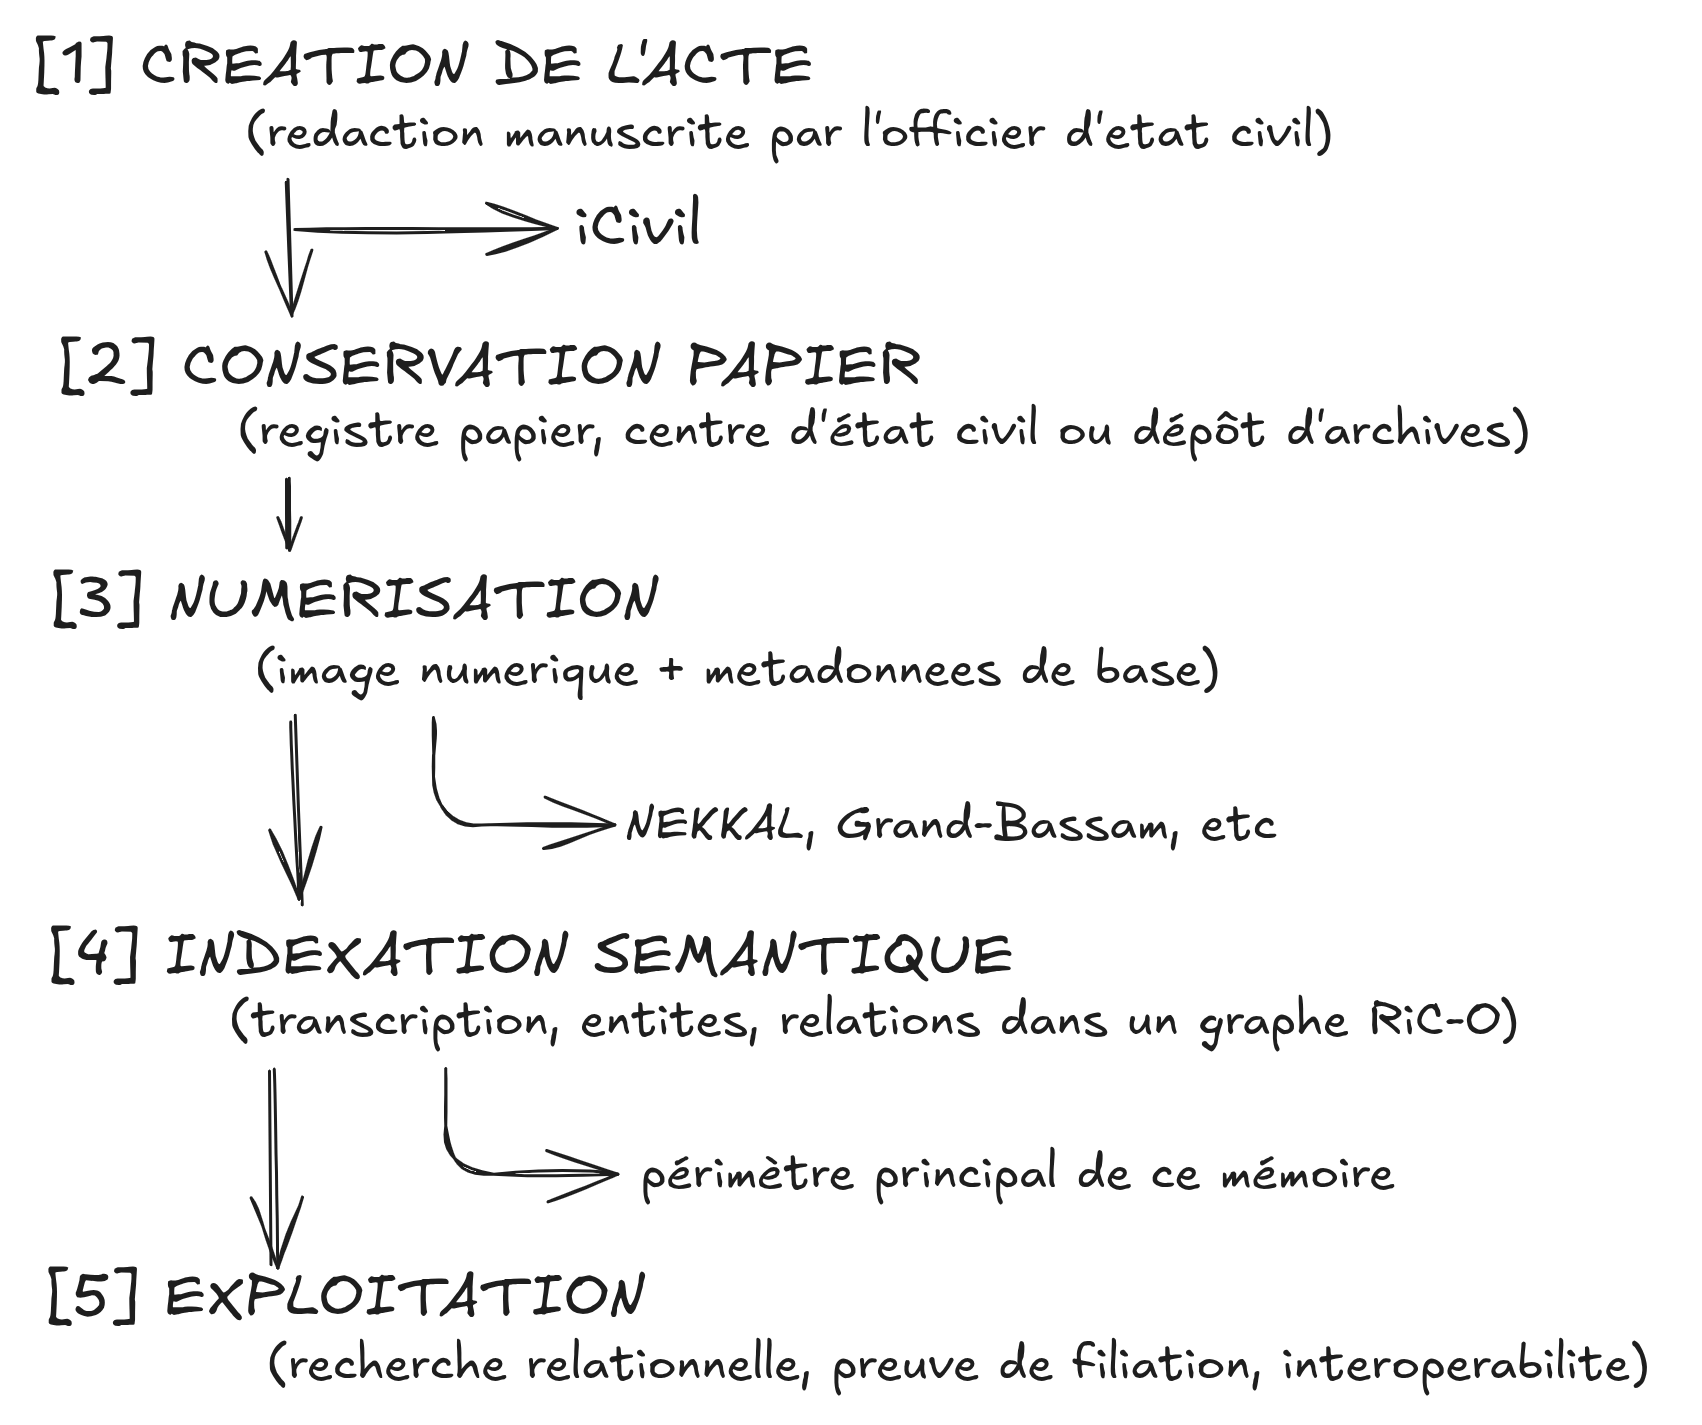
\includegraphics[width=0.8\textwidth]{figures/représentation_cycle_de_vie_acte.png}
    \caption{Cycle de vie de l'acte d'État civil et couverture des reformes actuelles. \textit{Source : l'auteur, réalisé avec Excalidraw}}
    \label{fig:lifecycle_of_registers}
\end{figure}

Ces deux démarches illustrent des modalités distinctes de déploiement progressif : expérimentation locale préalable à une éventuelle extension nationale dans le cas ivoirien, et projet de collecte et de conversion numérique à périmètre national dans le cas congolais.
Les sources consultées ne documentent toutefois pas de représentation sémantique des liens entre personnes et événements.
Le présent mémoire examine précisément la faisabilité d'une telle structuration pour les registres manuscrits.

Au Cameroun, la loi n\textsuperscript{o}~2024/001 du 24 juillet 2024 régissant les archives fixe un cadre général pour la gestion, la conservation, la sécurisation et la modernisation des archives \cite{cameroun2024loiarchives}.
Elle ne définit toutefois pas de chaîne opérationnelle spécifique de transcription, de résolution d'entités ou d'indexation sémantique des registres d'état civil manuscrits.
Ce mémoire examine précisément les conditions techniques et méthodologiques d'une telle exploitation.

Comme l'illustre la Figure~\ref{fig:lifecycle_of_registers}, les réformes examinées couvrent principalement l'enregistrement numérique, la numérisation et, dans certains cas, l'indexation documentaire.
Les sources publiques consultées ne décrivent pas de dispositif d'indexation sémantique reliant explicitement personnes, événements et actes.
Le mémoire se situe à ce niveau, en évaluant la transformation de registres manuscrits en données relationnelles, traçables et interrogeables.

\section{Les registres manuscrits d'état civil comme patrimoine documentaire}

Cette section examine les registres manuscrits comme objets matériels, administratifs et probatoires.
Leur état de conservation conditionne directement la qualité des images produites lors de la numérisation et, par conséquent, les performances des outils de reconnaissance automatique examinés en section 1.4.

\subsection{Diversité matérielle, scripturaire et enjeux de conservation}

Les registres d'état civil peuvent présenter des formats, supports, encres, écritures et formulaires variables selon les périodes et les lieux de production.
Les études consacrées aux manuscrits d'Afrique subsaharienne documentent des difficultés comparables de conservation, liées à la variabilité des supports et à leur vulnérabilité environnementale \cite{abdoulahi2019contribution,ala2005batiments}.
Ce rapprochement relève toutefois d'une analogie matérielle : les corpus diffèrent par leur fonction, leur langue et leurs conditions de production.

\begin{figure}[H]
    \centering
    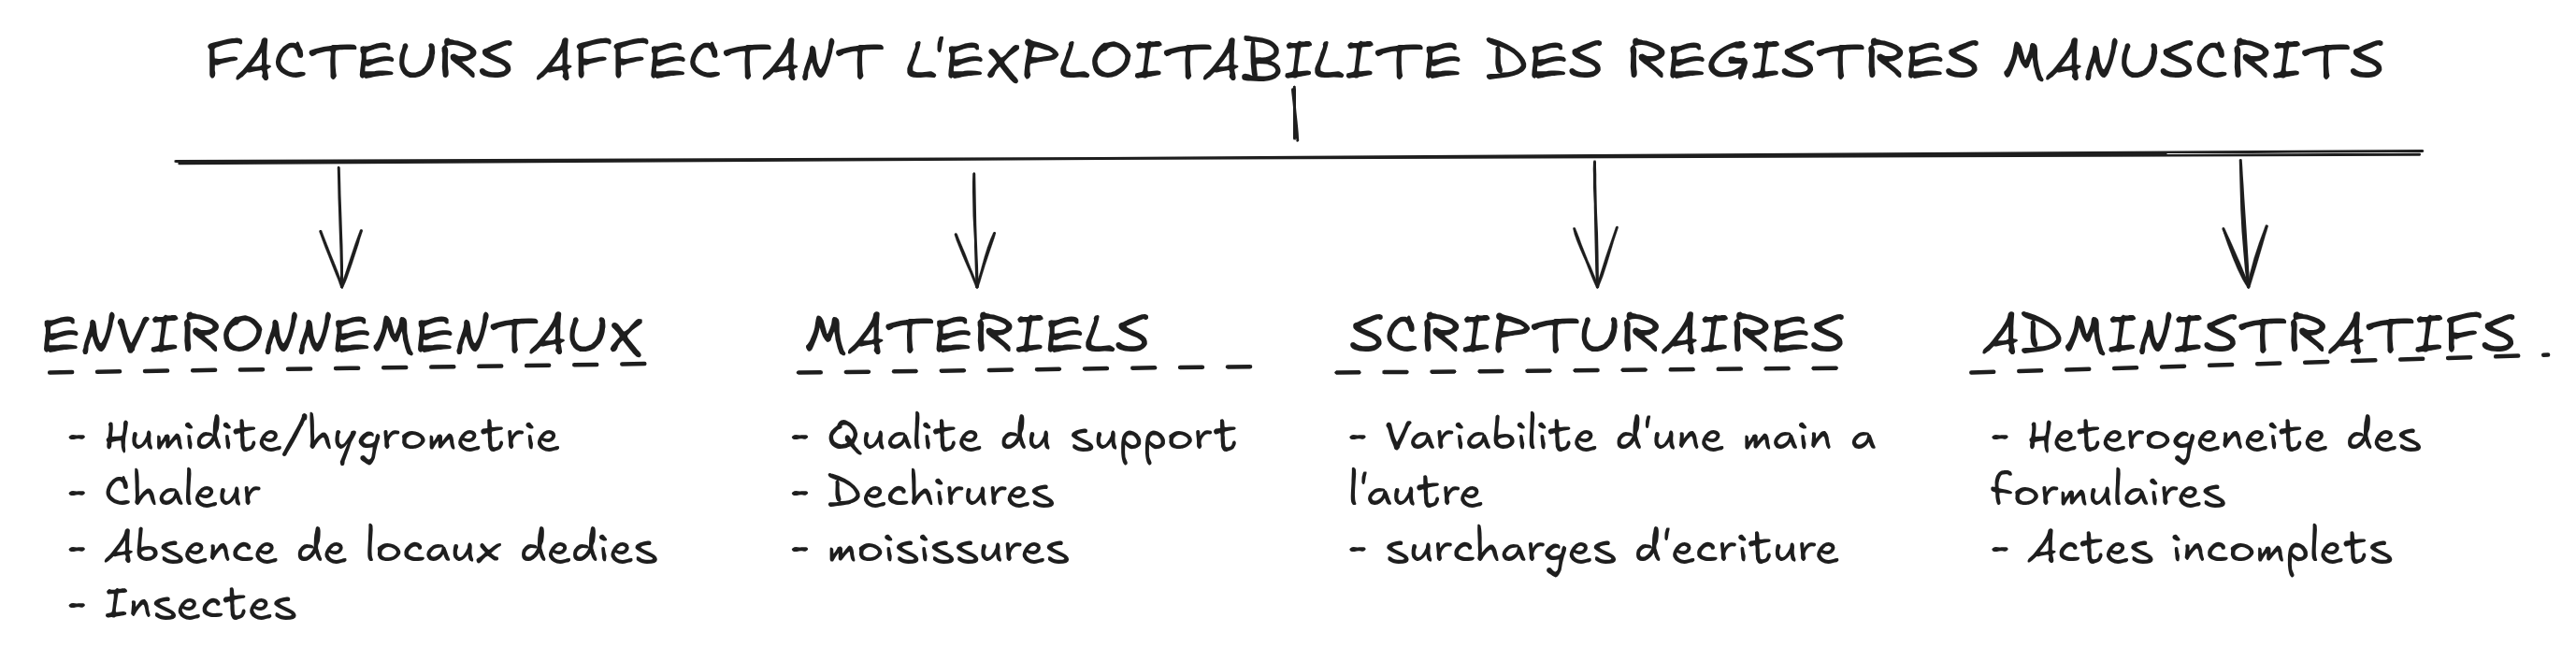
\includegraphics[width=0.99\textwidth]{figures/facteurs-exploitabilite.png}
    \caption{Facteurs affectant l'exploitabilité des registres manuscrits. \textit{Source : l'auteur, réalisé avec Excalidraw}}
    \label{fig:facteurs-exploitabilite}
\end{figure}

Dans les contextes où les conditions de conservation ne sont pas régulées, la température, l'humidité, les moisissures, les insectes et les manipulations répétées peuvent dégrader le papier et les encres.
Ces facteurs affectent la lisibilité des actes et augmentent la difficulté de leur transcription automatique.
Ils imposent donc de documenter, pour chaque corpus, l'état matériel des registres afin d'interpréter les résultats de reconnaissance et d'extraction.
La dégradation physique n'annule pas la valeur probatoire de l'acte, mais elle peut limiter son accessibilité et son exploitabilité.
La Figure~\ref{fig:facteurs-exploitabilite} synthétise les facteurs susceptibles d'affecter l'exploitabilité des registres.

\subsection{Valeur probatoire des actes anciens et préservation numérique en contexte de ressources limitées}

Les actes d'état civil anciens peuvent conserver une valeur probatoire durable lorsqu'ils restent authentifiables, intègres et rattachables à une autorité compétente.
Ils constituent des preuves importantes de l'identité juridique, de l'âge ou de la filiation, notamment en l'absence de documents contemporains \parencite{uneca2020status,un2023guidelines}.

La numérisation améliore l'accès aux registres fragiles, mais ne remplace ni leur conservation physique ni leur valeur juridique.
Les travaux consacrés à la préservation numérique dans les bibliothèques universitaires sud-africaines mettent notamment en évidence des difficultés de financement pérenne, de compétences spécialisées, d'obsolescence technologique et d'infrastructure \parencite{masenyaFactorsThatInfluence2020,masenyaDigitalPreservationPractices2019}.
Ces résultats fournissent un point de comparaison utile pour les institutions archivistiques disposant de ressources limitées, sans pouvoir être généralisés mécaniquement à tous les services d'état civil.

Dans cette perspective, la numérisation doit être distinguée de l'exploitation sémantique.
Le graphe de connaissances doit donc être conçu comme une couche sémantique dérivée, traçable et explicitement reliée aux actes sources.
L'enjeu n'est pas de remplacer l'acte original, mais d'en améliorer l'exploitabilité sans produire d'assertions non attestées.

\section{Standards et modèles de description archivistique}

Le choix d’un modèle de représentation adapté aux relations présentes dans les actes d’état civil suppose de distinguer les fonctions de préservation, de description hiérarchique et de description sémantique.
Cette section examine les principaux standards mobilisables avant de présenter RiC-O, retenu comme cadre de modélisation dans ce mémoire.

\subsection{Modèles classiques : OAIS, EAD et Dublin Core}

Le modèle OAIS (\textit{Open Archival Information System}), normalisé par l’ISO 14721, constitue un cadre de référence pour la préservation numérique.
Il décrit les fonctions d’un système d’archivage --- versement, stockage, gestion des données, administration, planification de la préservation et accès --- ainsi que les paquets d’information qui circulent entre elles.
OAIS éclaire donc l’organisation nécessaire à la conservation durable des archives, sans définir la représentation sémantique du contenu d'un document : il ne dit rien de la manière de représenter un acte de naissance et les personnes qu'il met en relation.
Sa pertinence pour ce mémoire est donc réelle mais indirecte —-- il éclaire les fonctions que devra assumer l'infrastructure de conservation, sans se substituer à un modèle sémantique du contenu.

EAD (\textit{Encoded Archival Description}) est un standard XML destiné à l’encodage des instruments de recherche archivistiques.
Il permet de décrire un fonds à plusieurs niveaux, du fonds à la pièce, selon une organisation généralement hiérarchique.
Il peut ainsi situer un acte dans son contexte de production et conserver des informations descriptives à son sujet.
Toutefois, EAD ne fournit pas, à lui seul, un modèle explicite d’entités persistantes permettant de relier, à travers plusieurs actes, un officier d’état civil, un déclarant, un enfant, des parents ou un événement selon des relations sémantiques typées.

Dublin Core propose un vocabulaire générique de métadonnées destiné à la découverte et à l’échange de ressources hétérogènes.
Dans sa version simple, il repose sur quinze éléments tels que le titre, le créateur, le sujet ou la date.
Ce niveau de généralité facilite l’interopérabilité minimale, mais demeure insuffisant pour distinguer systématiquement les rôles spécifiques intervenant dans un acte d’état civil.
Une propriété comme \texttt{creator} peut désigner une personne ou une organisation responsable de la ressource, sans exprimer nécessairement la fonction précise exercée dans l’acte.

Pris isolément, OAIS, EAD et Dublin Core répondent donc à des besoins complémentaires : préservation du système, description hiérarchique des fonds et découverte de ressources.
Ils ne fournissent toutefois pas un modèle archivistique complet permettant de représenter explicitement les relations entre les personnes, les événements et les actes d’état civil.
Cette limite motive l’étude d’une approche fondée sur RiC-O.

\subsection{Records in Contexts et l’ontologie RiC-O : principes, structure et interopérabilité}

Développé par le Groupe d’experts en description archivistique (EGAD) du Conseil international des archives depuis 2012, le standard \textit{Records in Contexts} (RiC) a été conçu comme un successeur des quatre normes descriptives antérieures de l’ICA : ISAD(G), ISAAR(CPF), ISDF et ISDIAH.
Il vise à les articuler dans un cadre conceptuel commun, centré sur les entités archivistiques et leurs contextes plutôt que sur des descriptions produites séparément.

RiC comporte quatre parties complémentaires : les fondements de la description archivistique (RiC-FAD), le modèle conceptuel (RiC-CM), l’ontologie (RiC-O) et les lignes directrices d’application (RiC-AG).
Les versions 1.0 de RiC-FAD, RiC-CM et RiC-O ont été publiées fin 2023 ; RiC-AG demeure en cours d’élaboration \textbf{ica2023ricrelease,ica2025ricwebinar}.
RiC-O, dans sa version 1.1, est une ontologie OWL 2 qui formalise RiC-CM et fournit un vocabulaire ainsi que des règles formelles pour produire des jeux de données RDF décrivant des ressources archivistiques et leurs contextes \parencite{icaegad2025rico11,clavaudica}.

L’apport de RiC-O tient à sa modélisation orientée entités-relations.
Documents, agents, lieux, événements, activités et règles de gestion peuvent être représentés comme des entités distinctes et reliés au moyen de propriétés explicites.
Un acte de naissance peut ainsi être décrit à la fois comme une ressource archivistique, comme la trace d’un événement et comme un document associé à plusieurs agents exerçant des rôles différents.
Cette approche ne résout pas automatiquement l’identification des personnes ni l’extraction du contenu manuscrit ; elle fournit le cadre nécessaire pour représenter, documenter et interroger les relations établies à partir des actes.

Les jeux de données produits en RDF peuvent être reliés à d’autres vocabulaires et référentiels, puis interrogés au moyen de SPARQL lorsqu’ils sont stockés dans une infrastructure compatible.
L’interopérabilité effective dépend toutefois des choix de modélisation, de la stabilité des identifiants, des règles de transformation, de la provenance des assertions et de la gouvernance des données.
RiC-O constitue ainsi un cadre de référence, non une solution technique complète de peuplement ou d’exploitation d’un graphe.

\subsection{Profils d’application RiC-O : état des lieux}

RiC-O est une ontologie générique : son application à un domaine particulier suppose de sélectionner les classes et propriétés pertinentes, de définir des contraintes d’usage et, si nécessaire, de documenter des extensions.
Les futures lignes directrices RiC-AG ont précisément vocation à fournir aux professionnels et aux développeurs des recommandations et des exemples de mise en œuvre de RiC-CM et RiC-O \textbf{ica2023ricfad}.

Les démonstrations actuellement disponibles portent principalement sur la conversion ou l’exploitation de métadonnées archivistiques existantes, notamment issues d’EAD, d’EAC-CPF ou de METS.
Elles ne constituent pas nécessairement des profils de production applicables tels quels à l’état civil.
Dans les ressources consultées, aucun profil RiC-O spécifiquement consacré aux registres d’état civil manuscrits, et a fortiori aux corpus d’Afrique subsaharienne, n’a été identifié.

Cette lacune ne signifie pas que le domaine est absent de RiC-O : le standard fournit des mécanismes génériques pour représenter des documents, agents, événements, lieux et relations.
Elle indique plutôt que les règles d’application propres à l’état civil --- modélisation de la filiation, distinction des rôles, gestion des actes associés, traitement des informations incertaines et provenance des assertions --- restent à définir et à évaluer.
C’est dans cet espace que s’inscrit l’objectif scientifique OS2 du mémoire.


\chapter{Méthodologie et cadre conceptuel}
\label{chap:methodologie}

\include{chapters/chap3_impl}
\chapter{Expérimentation, Résultats et Évaluation}
\label{chap:experimentations}
\chapter*{Conclusion générale et perspectives}
\addcontentsline{toc}{chapter}{Conclusion générale et perspectives}
% Conclusion générale à venir

% --- Bibliographie ---
\printbibliography[heading=bibintoc, title={Bibliographie}]

% --- Annexes ---
\appendix
\chapter{Annexes}
\label{chap:annexes}
% Annexes à venir

\end{document}